\documentclass[10pt]{article}
\usepackage[margin=.82in]{geometry}
\usepackage{xeCJK,booktabs,graphicx,amsmath,hyperref,microtype}
\IfFileExists{.local_fonts/CJK-Regular.ttf}{\setCJKmainfont[Path=.local_fonts/,BoldFont=CJK-Bold.ttf]{CJK-Regular.ttf}}{\setCJKmainfont{Noto Serif CJK SC}}
\hypersetup{colorlinks=true,urlcolor=blue,pdftitle={CounterScene-3D Chinese Edition},pdfauthor={CounterScene-3D Contributors}}
\setlength{\parindent}{0pt}\setlength{\parskip}{5pt}
\title{CounterScene-3D：具有状态延续的原生素材空间评测}
\author{CounterScene-3D Contributors}\date{}
\begin{document}\maketitle
\begin{center}\small\href{report.pdf}{English edition}\end{center}
\begin{abstract}
本中文版本与英文主报告使用同一冻结数据、图表和评测口径。CounterScene-3D 评测模型在观察变化后，通过可执行程序操作实际三维素材的能力。五类任务包含三十个开发实例、六十个有序操作。我们比较两个参测模型，独立检查几何与运动结果，使用 Astra 提供辅助视觉评分，并通过小模型 best-of-four 实验分析奖励信号。结果只适用于当前几何开发集，不代表真实机器人可靠性或分布外泛化。
\end{abstract}
\section{基准设计与决策递进}
空间任务不能只检查最终画面是否合理。评测保存观察、程序、实际执行状态、工具反馈和不可撤销的提交，防止最终场景掩盖先前错误。
每类任务包含两个场景种子和 L1--L3 三个层级，共六个实例。各层级分别要求一、二、三个有序操作；A 类对应 k06、k14、k34。递进来自新的工作要求、观察更新与已完成工作的保留，而不是输入更长或在两个近似场景间反复切换。难度仍是经验问题，更多阶段不保证模型成功率严格下降。

\textbf{A：搬移与恢复。} 第一阶段将工作台明显移到另一位置，并将台面物品暂放在原位置地面；第二阶段按原台面相对偏移恢复物品；第三阶段处理另一工作区，同时保留前面成果。评分检查明确目标、支撑和保留要求，只有无碰撞还不够。

\textbf{B：逐步修复碰撞。} 每阶段只开放当前工作区，保留已修复区域与尚未开放区域。中间阶段允许明示的待修复问题，最终必须满足完整硬约束与可行软约束。模型须指认不可满足的软约束。固定 gold 后续方案失败不等于不存在其他可行后续方案。

\textbf{C：变化视角下的重建。} 初始提供实际素材样例和标定的正、侧、俯视图。后续目标明显移动物体，并释放新的斜视观察，要求模型修正位置与允许的尺度，同时保留仍正确的结构。额外视角受查询预算限制；公开视角吻合并不能替代隐藏视角和物体中心误差检查。

\textbf{D：连续操控。} 每阶段抓取不同物体、放到柜子上、释放并移动到后续位置。下一阶段继承实际末端关节和已释放物体的位置，已释放物体成为障碍。抓取失败不会自动搬动物体，释放位置来自实际执行的末端位置。模型还必须处理关节零点偏移。

\textbf{E：误导反馈。} 逐步修复真实物理问题，同时面对错误通过、错误失败、遗漏、数值噪声或被隐藏的碰撞信息。模型可测量实际几何。几何修复与检查器故障诊断分别报告，未实际出现在冻结实例中的干扰类型不算已评测。
\begin{figure}[htbp]\centering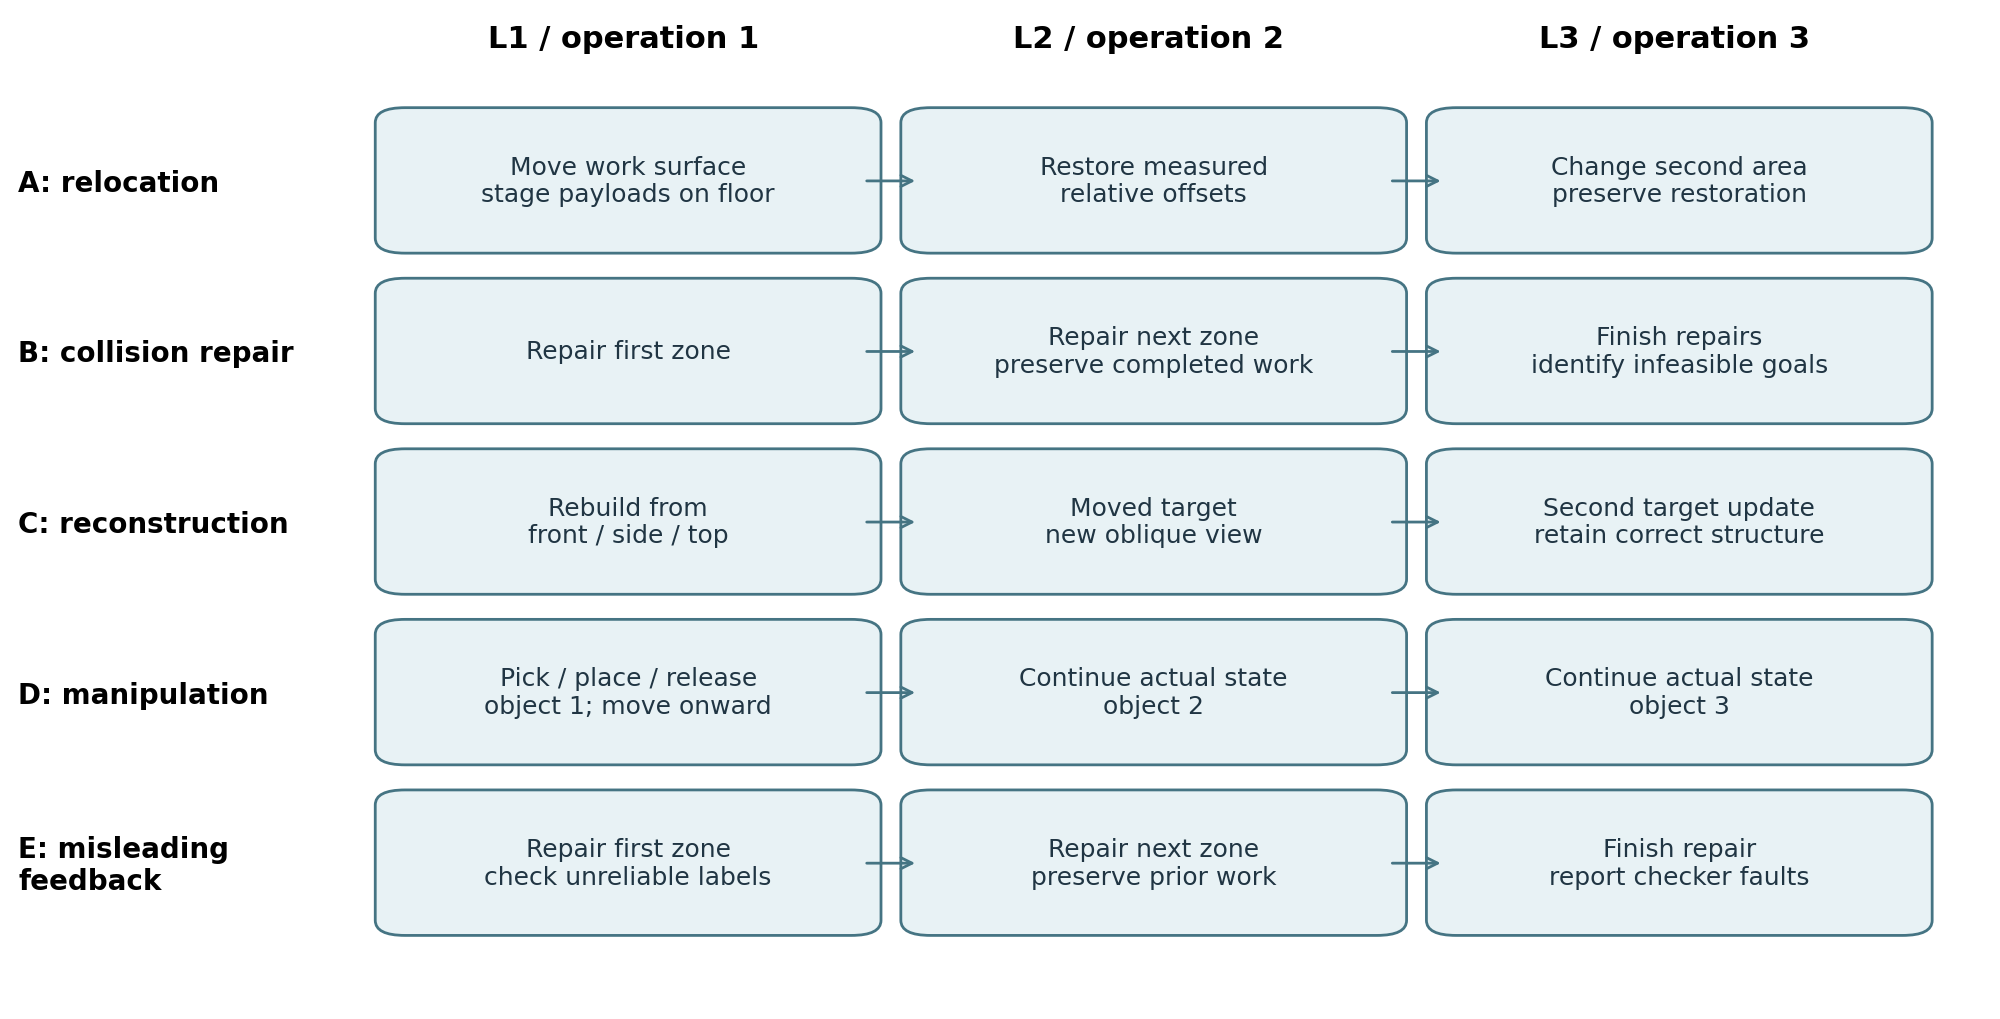
\includegraphics[width=\linewidth]{figures/benchmark_design.png}\caption{五类任务的实际阶段依赖。后续操作必须保留此前成果。图中英文术语与主报告一致。}\end{figure}
\section{执行、约束与端到端验证}
输出是受限 Python 的 build 函数，返回完整素材位姿或机械臂控制序列。解释器允许有界算术与集合操作，禁止导入、属性访问、文件和网络访问。公开参数不包含隐藏目标。素材身份固定，模型操作的是实际网格；包围盒不能替代展示或静态评估中的素材。

所有实例从内容绑定的阶段文件加载。Gold 通过实际执行验证硬约束、共同可行的软目标、支撑、边界、接触和穿模。捷径测试包括旧答案复用、仅更新固定物体坐标、忽略新观察和不适当复用早期运动方案。这些是具体反例与可行见证，并非对所有策略的完备证明。

搬移与重建目标变化的路径检查使用实际连通网格导出的包络。机械臂另外检查连续的臂、工具、携带物体、固定设施和已释放物体间净空、关节限制与抓放语义。包络重叠表示未能证明安全，不自动等于实际网格相交。该模型是运动学模型，不模拟摩擦、力闭合、扭矩或动态稳定性。静态修复任务主要评价端点，不能将其可视化误认为已验证运输路径。

严格整条轨迹成功要求每个必需阶段、当前约束和此前成果都正确。有效但错误的提交不可撤销，不能用一个正确末态抹去早期失败。C 还要求隐藏视角的逐物体平均轮廓 IoU 至少 0.8，且每个原生物体包围中心误差均不超过 0.05 米。平均值可能隐藏某个小物体的大误差，因此两项必须同时满足。D 必须满足连续有效性和实际事件顺序。

基础设施错误与模型失败分开。已确认响应精确重放而不重新生成，复用响应只计一次。程序字节与原生素材哈希保留身份。
\begin{figure}[htbp]\centering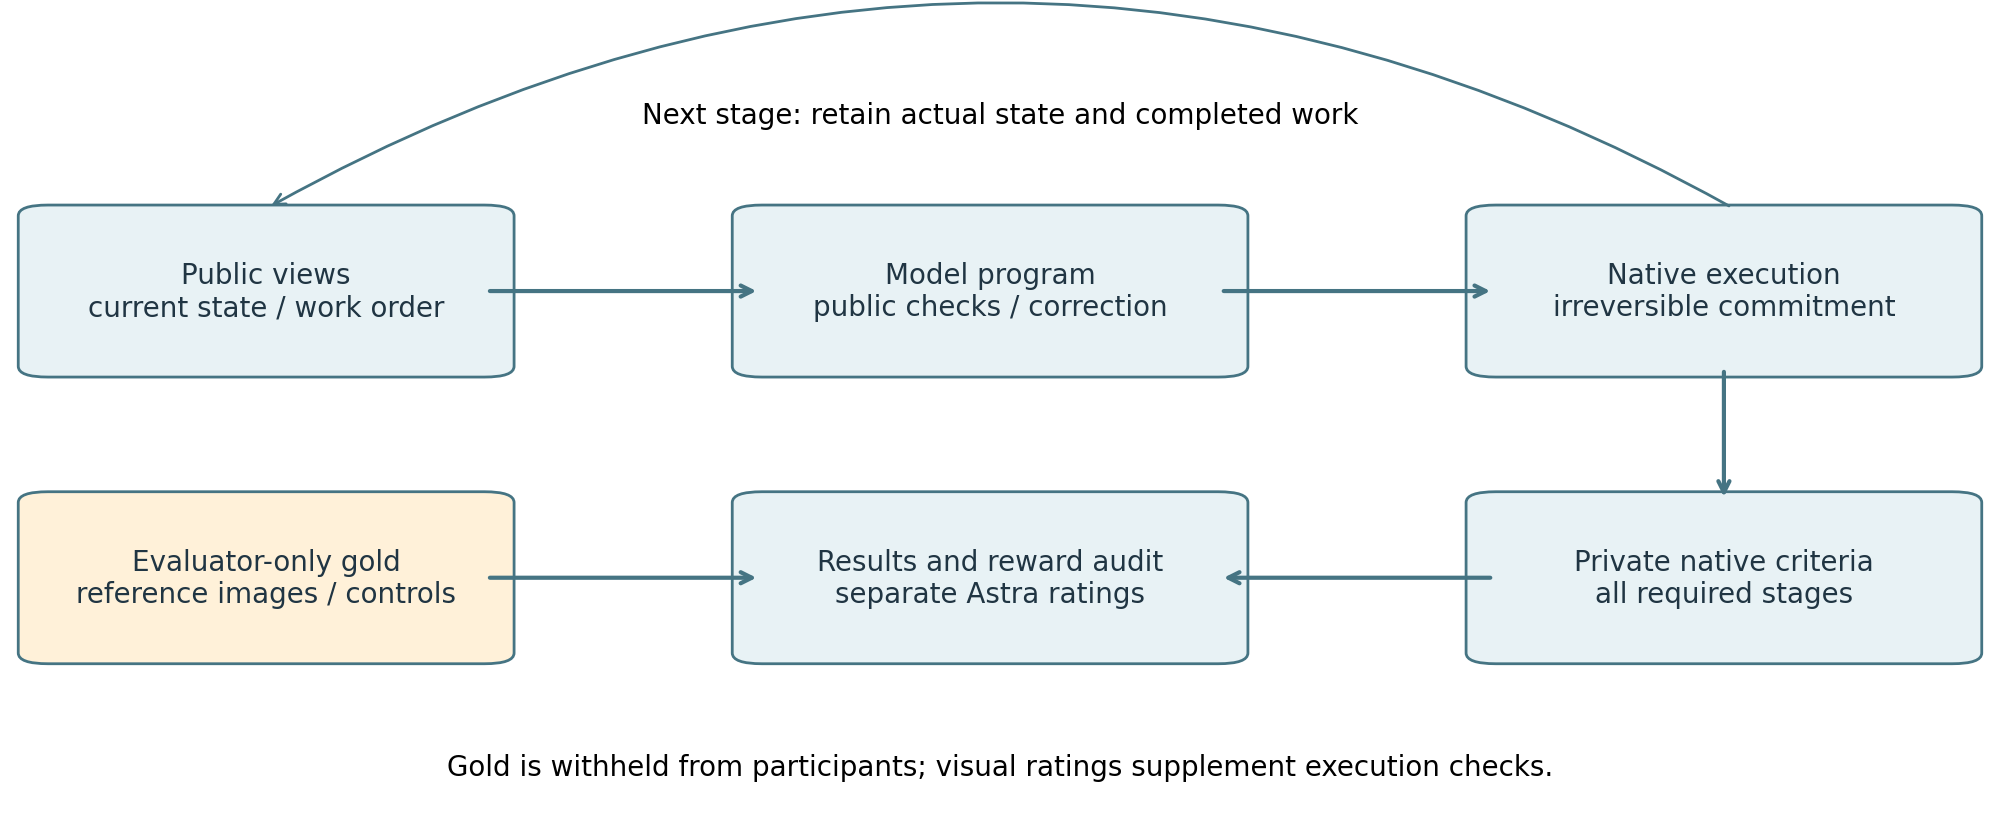
\includegraphics[width=\linewidth]{figures/evaluation_flow.png}\caption{评估流程：公开观察驱动模型行动；隐藏程序和度量目标仅由评估器使用；视觉评分不能覆盖执行检查。}\end{figure}
\section{参测协议与完整结果}
参测模型为 GPT-6.1 Sol 与 Claude Opus 5.5，使用 medium reasoning，每个响应最多 8,000 输出 token，每个操作最多十四个动作。三十个实例乘两个模型形成六十条基础轨迹；固定 L3 面板为每类任务和每个模型再增加一次独立生成，共七十条。每组只有两次生成，方差估计仅有一个自由度，不足以形成稳定的不确定性估计。可选反馈和视角消融在执行前取消，基础覆盖和离线捷径控制完整保留，不能据此声称消融的因果效果。

全部七十条轨迹均具备有效基础设施证据。下表只汇总基础比较，每个任务和模型有六个实例。GPT 严格成功 26/30，Claude 为 24/30；这是开发集描述，而非普遍优劣结论。
\begin{center}\begin{tabular}{llrrr}\toprule 任务 & 模型 & 样本 & 严格成功率 & 形状奖励 \\\midrule
A & Claude & 6 & 1.000 & 1.000 \\
A & GPT & 6 & 1.000 & 1.000 \\
B & Claude & 6 & 0.833 & 0.982 \\
B & GPT & 6 & 0.833 & 0.981 \\
C & Claude & 6 & 0.333 & 0.432 \\
C & GPT & 6 & 0.500 & 0.580 \\
D & Claude & 6 & 1.000 & 1.000 \\
D & GPT & 6 & 1.000 & 1.000 \\
E & Claude & 6 & 0.833 & 0.765 \\
E & GPT & 6 & 1.000 & 0.912 \\
\bottomrule\end{tabular}\end{center}
\begin{figure}[htbp]\centering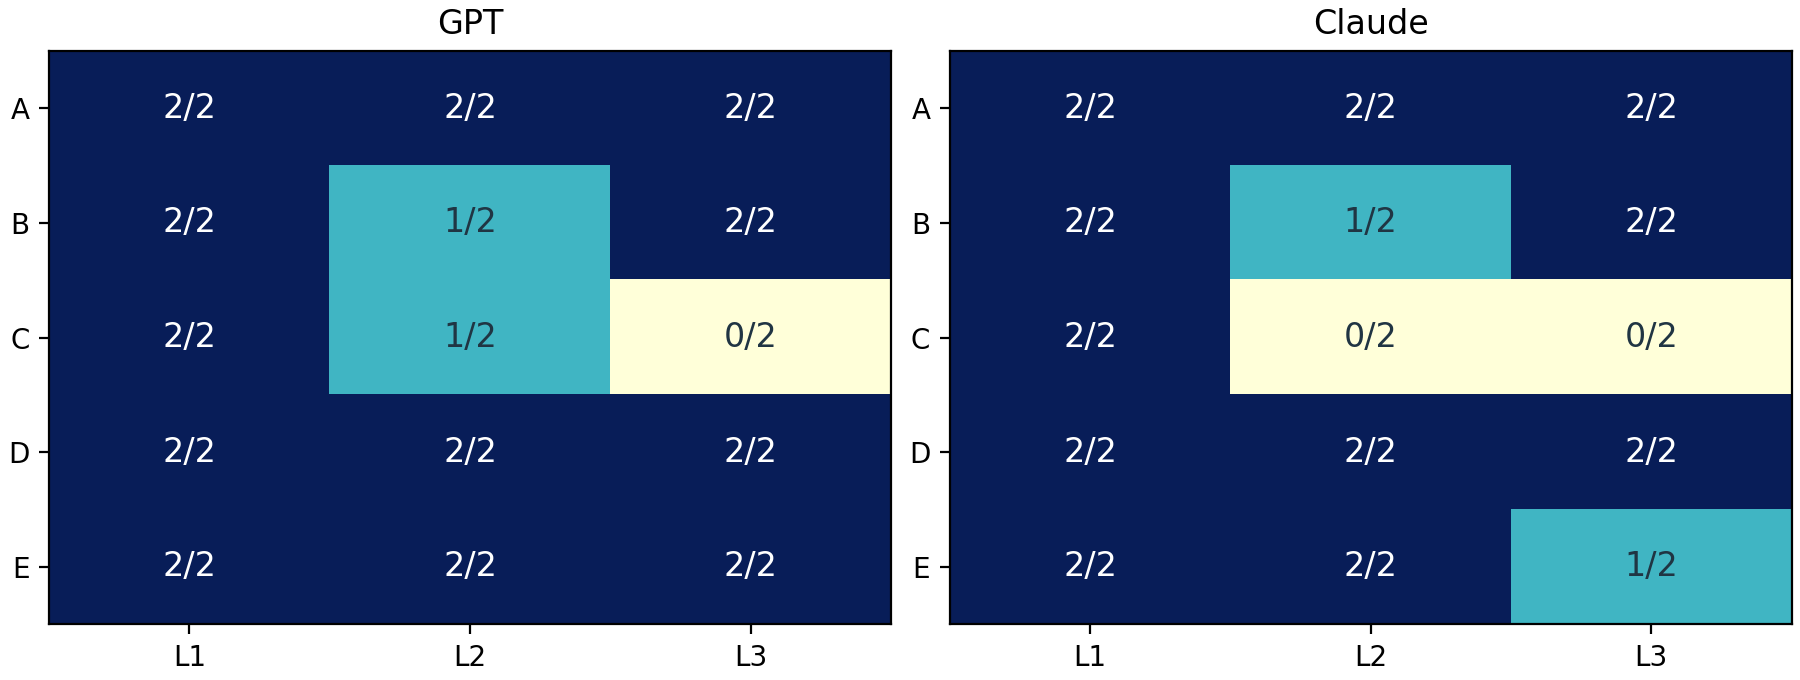
\includegraphics[width=.9\linewidth]{figures/performance_by_level.png}\caption{每个格子对应两个种子的严格成功数。任务难度不是关于层级的简单单调排名。}\end{figure}
\textbf{共享盲点。} B-L2-s0 中两个模型都在公开检查器报告硬约束失败后，提交未改变的程序。前一阶段成功，最终关系修复失败。这里能观察到的是未利用反馈修正，而不是模型的内部意图。

\textbf{更新失败。} C-L2-s0 中 Claude 第一阶段重建成功，目标变化后未通过隐藏视角与度量检查。第二阶段执行十三个动作，没有额外视角查询。不能据此推断额外查询必然解决问题。

\textbf{视觉与物理分离。} GPT 在 C-L2-s1 第一阶段通过轮廓与中心检查，却保留实际物理冲突；第二阶段成功仍不能消除早期失败。Claude 在该实例也有物理冲突，并额外存在度量问题。

\textbf{修复与诊断分离。} E-L3-s1 中 GPT 满足 26/26 个原生关系，识别 2/4 个检查器故障；Claude 满足 25/26，识别 0/4。几何成功不代表完整诊断。分类允许一条轨迹出现多个问题，工具错误也可能出现在最终成功的轨迹中。
\begin{figure}[htbp]\centering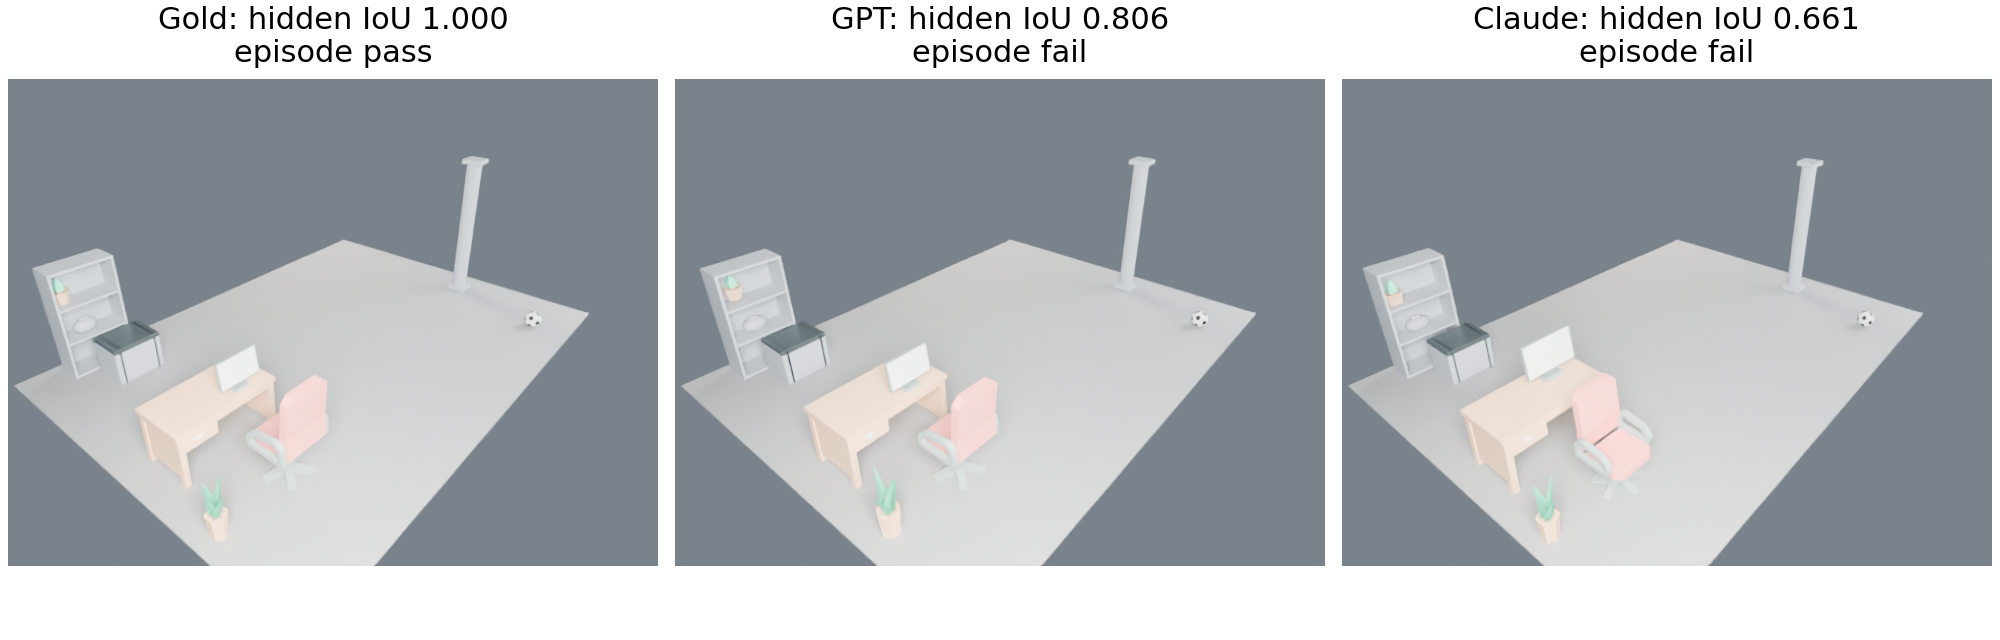
\includegraphics[width=\linewidth]{figures/reconstruction_comparison.png}\caption{C-L3-s0 的真实参考与模型渲染。IoU 来自隐藏视角；通过视觉阈值不保证物体中心、物理检查或整条轨迹通过。}\end{figure}
\section{奖励是否适用于强化学习}
每阶段确定性奖励要求物理许可的功能成功。形状奖励对适用的功能、约束、可行软目标、保留、诊断、操作、重建和运动分量取等权平均。整条轨迹按必需阶段数平均，未执行阶段记零；不适用维度不当成零填入。未获许可的物理问题或移动锁定对象会触发门控。运动经过某个路标不能抵消路径不安全。

校准包含三十个实例、四类输出和三次重复，共 360 次数值评分。Gold、空输出、旧答案或静止输出、安全中间解测试已声明的排序，全部通过；固定数值重算的最大奖励方差为零。全部六十个有序 gold 阶段也取得满分，包括允许暂留指定问题的中间阶段。另取每类任务一个 GPT 输出，使用任务包独立执行第二次，完整阶段评分一致，配对奖励方差为零。这个五输出、每输出两次的原生重跑子集，不代表所有输出或所有平台稳定。

十组独立生成面板的形状奖励总体方差介于 0 与 0.2223。这与重算同一输出的方差不同，样本量很小。Astra 固定图像重复评分的样本方差介于 0 与 0.0093，控制样本平均可评分覆盖率为 0.906；不确定项为缺失，而非失败。五类任务的弱排序均满足，且 gold 均严格高于旧答案，但平分仍削弱区分度。七个功能失败的基础输出获得至少 0.75 的辅助视觉分数，说明视觉合理性不能替代执行检查。

Astra 只作为匿名视觉辅助评估器，比较参考与候选的身份布局、可见支撑、可见净空和可见目标吻合。D 使用代表性轨迹中段帧；静态图像无法证明整条路径、终点事件或抓放正确性。同一提供方与其中一个参测模型有家族关联，也需要警惕潜在偏差，不能用单个评估器估计因果偏差。

小模型实验使用量化 Qwen3.5:9B（Q4\_K\_M），每个任务两个开发实例、每池四个固定种子候选，共十池四十个候选。选择只依据公开工具奖励，再独立审计隐藏质量；失败和相同分数均保留，平分选首个候选。平均隐藏质量由首个候选的 0 提高到选择后的 0.2，改善仅来自 A。E 的选择后公开分数为 0.3、隐藏质量为 0；若未比首个候选提高公开分数，就不能宣称优化学会了利用漏洞。这是 best-of-four 推理实验，不是 RL 训练或泛化证明。
\begin{figure}[htbp]\centering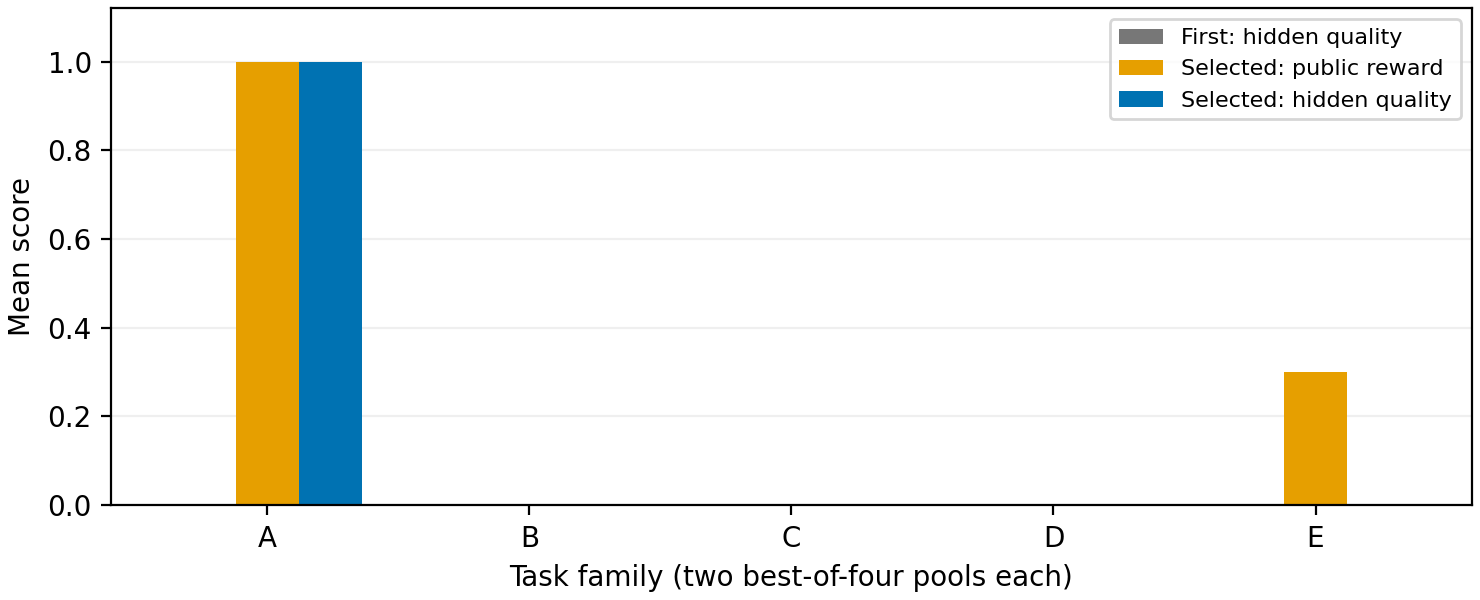
\includegraphics[width=.9\linewidth]{figures/qwen_reward_quality.png}\caption{公开奖励负责选择，隐藏质量负责独立审计。只有 A 在该小样本中改善，其他任务仍为零隐藏质量。}\end{figure}

各维度分析分别讨论空程序、素材替换、接触容差、保留低编辑成本却放弃目标、信任错误标签、轮廓掩盖度量误差，以及用漂亮端点隐藏不安全路径。对应分类为难以利用、可利用但有边界、或软性视觉判断。原生网格、联合中心条件、操作目标、锁定状态和事件检查针对具体攻击，但容差和观察不完整仍存在边界。

我们不会把当前标量奖励用于不受限制的 RL。原生许可检查提供有限保障，而视觉相似性和检查器一致性仍是代理。Best-of-four 能检验选择质量，不能证明训练稳定性或抵抗自适应策略的能力。
\section{复现、局限与改进方向}
任务包将公开提示与图像同评估器目标、gold 和评分代码分离。原生素材保留许可与内容哈希。无需提供方访问或模型权重即可重算数值；原生重放需要 Python 与外部 Blender。单命令核对奖励、表格、生成方差、视觉评分和候选选择，另可执行全部保留动作。五个任务包的 gold 均独立验证可解。报告和网页使用同源数值，不把基础设施缺失算为模型零分。

公开开发证据包含有序事件哈希、实际代码修改提交与英文提示派生稿。完整可见事件日志另留本地；内部推理与配置数据排除，私密正文不公开。网页区分 gold、模型实际执行和未执行阶段。轨迹来自实际关节状态，播放速度仅用于说明。

\textbf{覆盖范围。} 两个世界种子和开发模板限制推断；后续应保留未见场景与更多素材目录，并扩展独立重复，再讨论模型排名。

\textbf{物理近似。} 保守包络可能误拒可行路径，几何支撑不等于动态稳定。应先用独立网格测试校准误拒，再加入力、摩擦和抓取动力学。

\textbf{视觉评分。} 单一模型家族并非人工真值，D 中段图片也不证明最终事件。应增加匿名独立评估器、人工抽查和短运动片段，检验事件敏感的判断。

\textbf{奖励有效性。} 等权分量是设计选择；应比较不同权重，进行更长的自适应攻击，并用留出质量审计。十个开发候选池不能证明 RL 稳定性，gold 重放也不证明规则完备。
\begin{figure}[htbp]\centering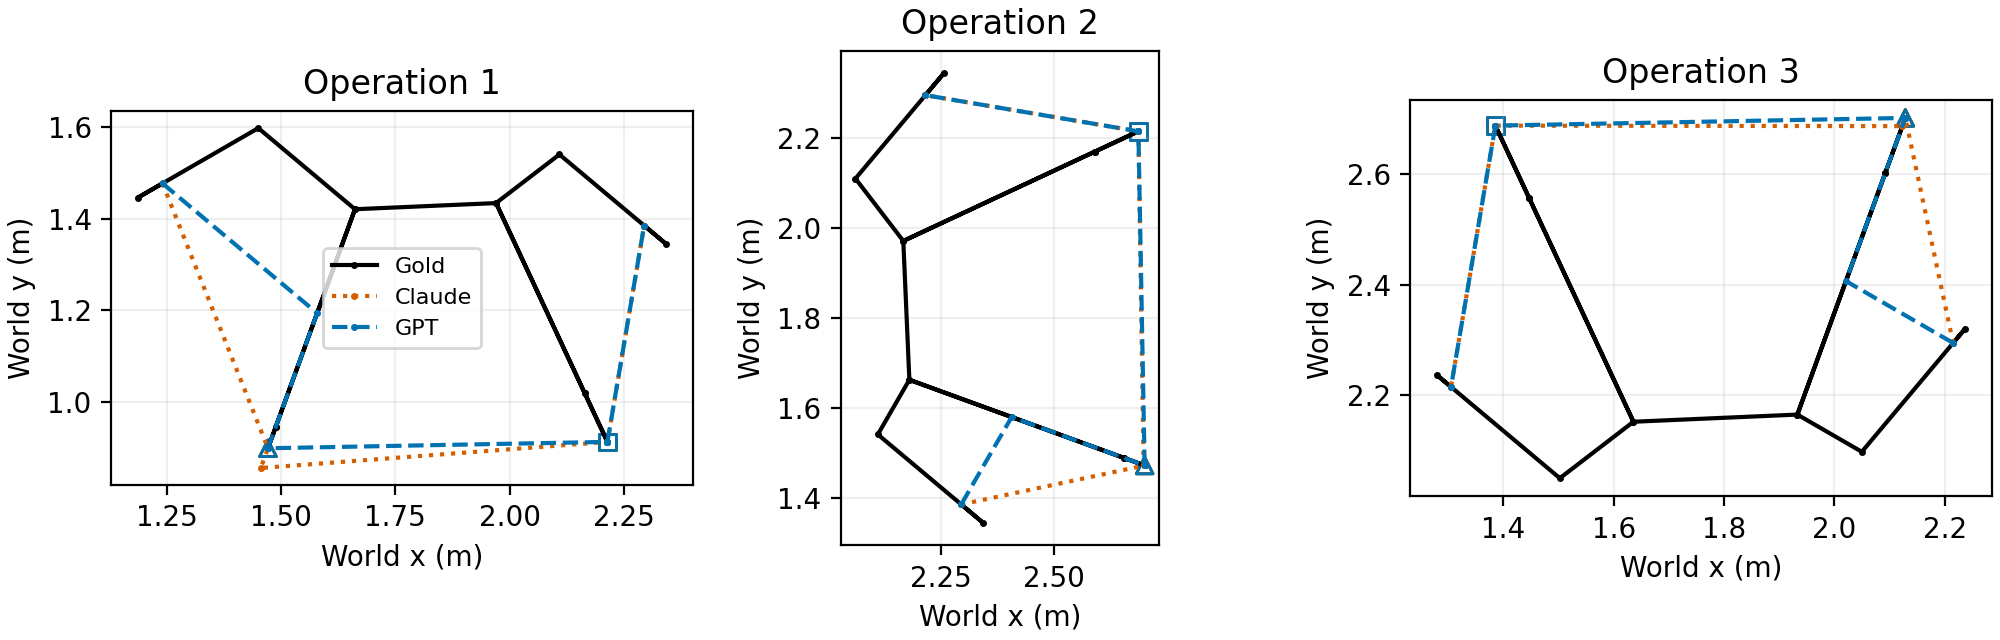
\includegraphics[width=\linewidth]{figures/motion_comparison.png}\caption{D-L3-s0 的实际末端轨迹关键帧，比较 gold、GPT 与 Claude。三角标记抓取，方形标记释放；连续安全依赖独立运动学证书，而非图上线段。}\end{figure}
\begin{figure}[htbp]\centering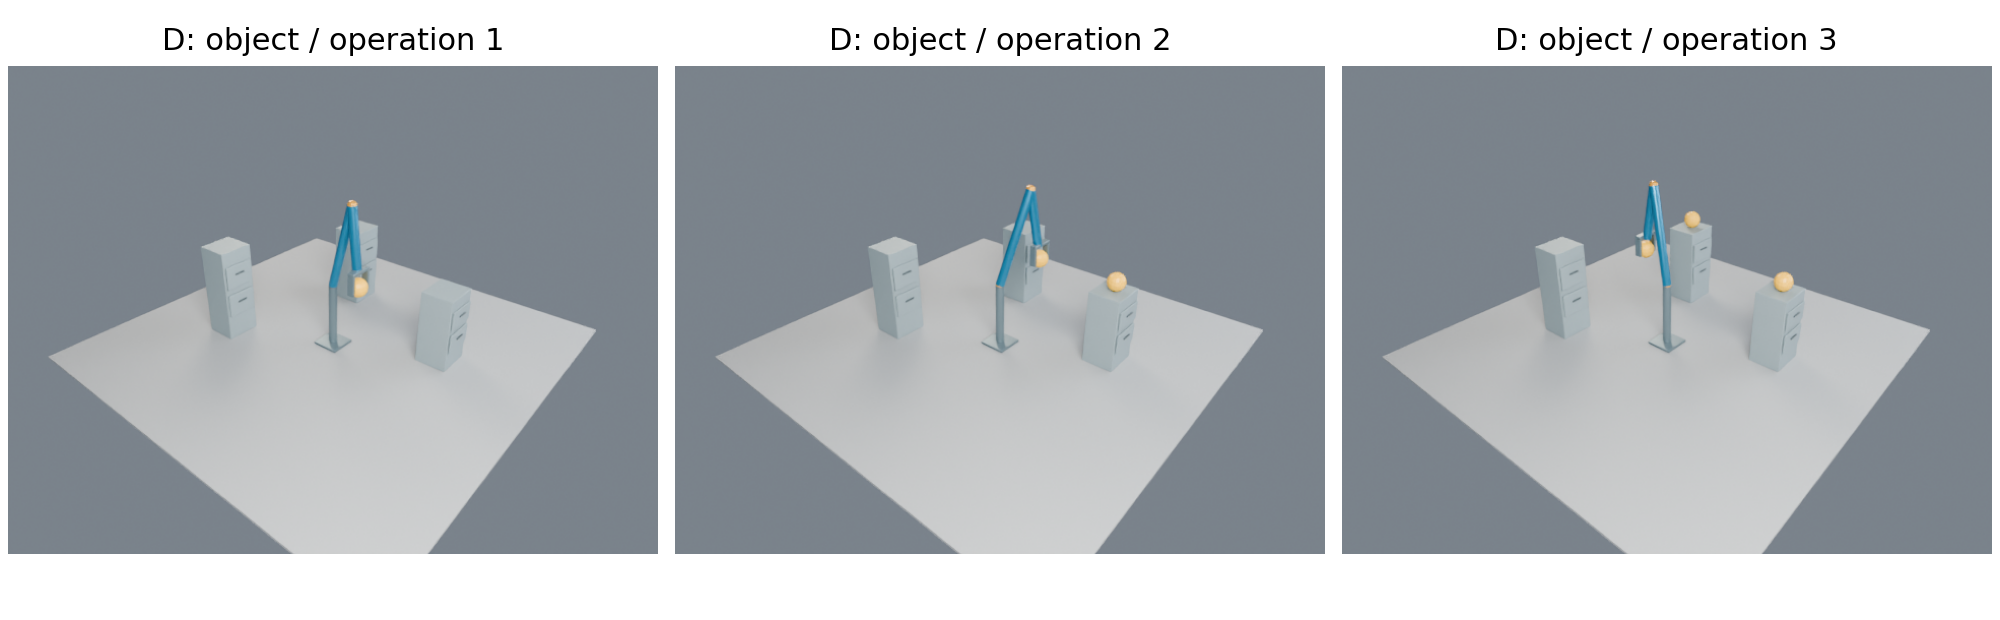
\includegraphics[width=\linewidth]{figures/motion_native_examples.png}\caption{D 的连续 gold 操作中段帧。后续画面保留先前释放物体；终点与事件语义须结合完整三维轨迹和原生检查。}\end{figure}
\clearpage\section{更多基准样例}
\begin{figure}[p]\centering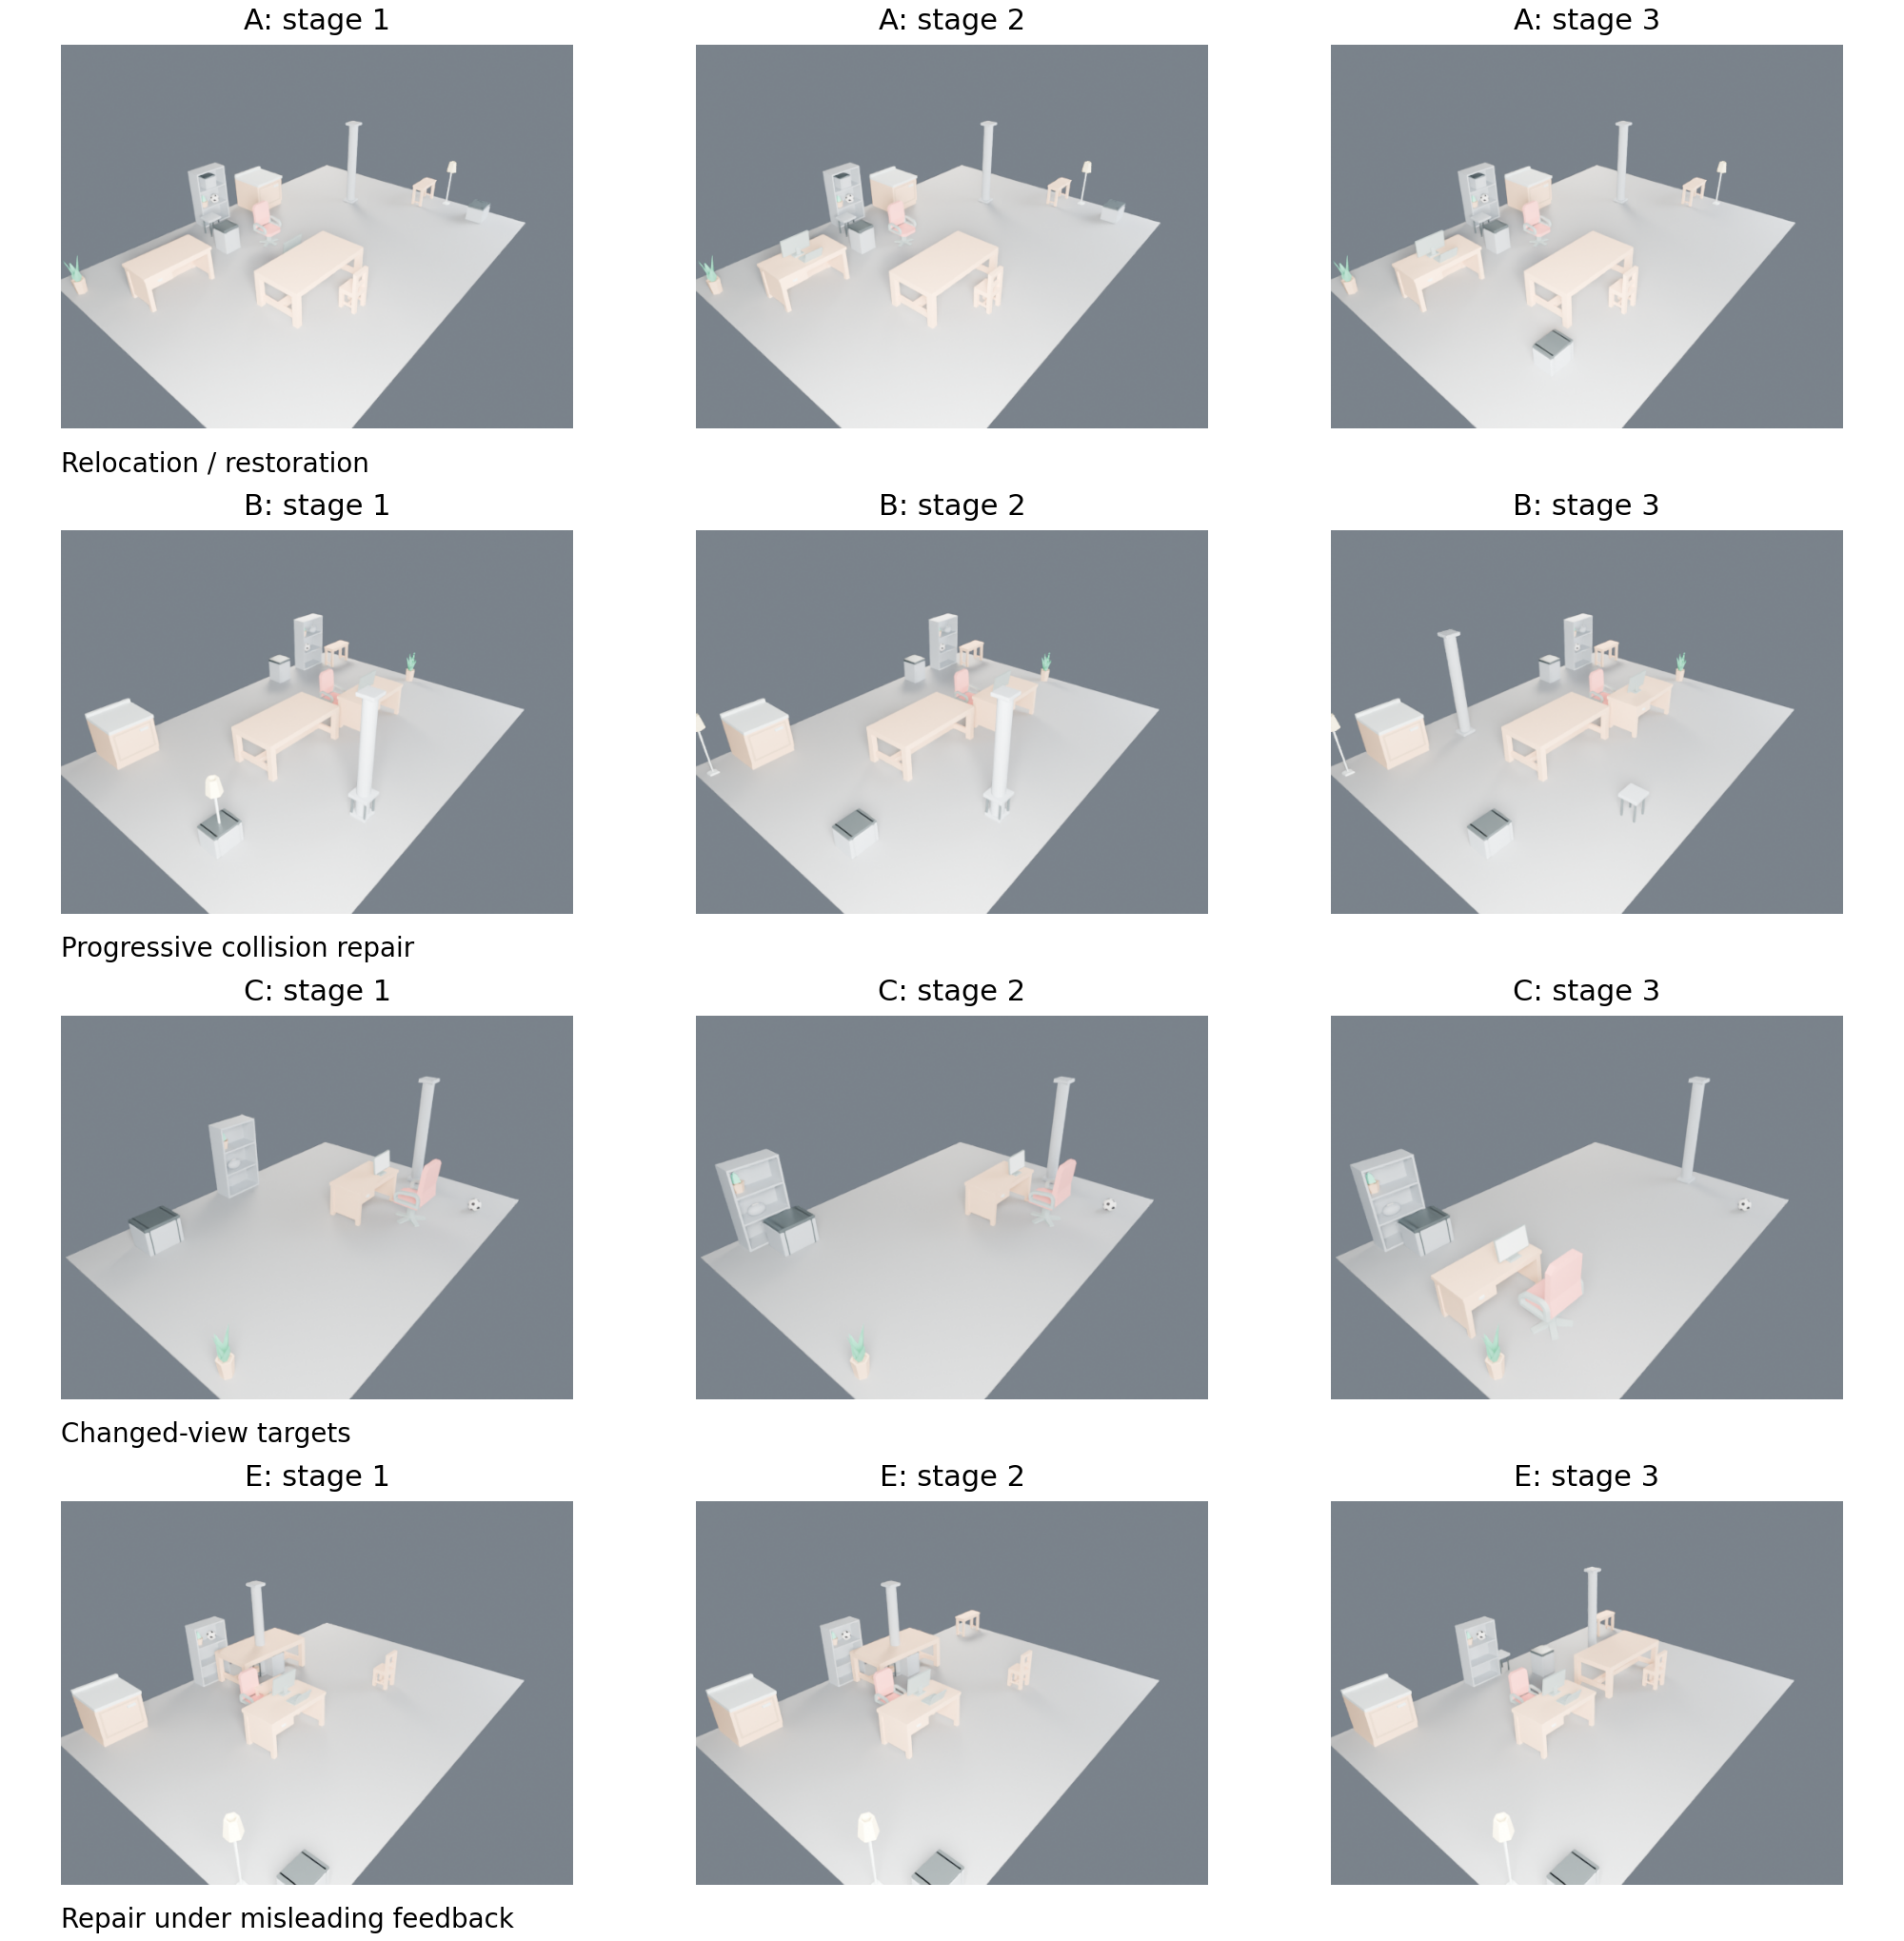
\includegraphics[width=.98\linewidth,height=.8\textheight,keepaspectratio]{figures/benchmark_examples.png}\caption{A、B、C、E 各三阶段的真实 gold 样例，使用种子零。B/E 中间阶段有意保留已声明的未来问题。这些是可行参考见证，不是模型输出。}\end{figure}
\end{document}
